\documentclass[12pt,a4paper]{report}
\usepackage[utf8]{inputenc}
\usepackage[spanish]{babel}
\usepackage{amsmath}
\usepackage{amsfonts}
\usepackage{amssymb}
\usepackage{graphicx}
\usepackage{multirow}
\usepackage[left=2cm,right=2cm,top=2cm,bottom=2cm]{geometry}
\usepackage{listings} %Inserta código en el archivo
\usepackage{graphicx} %Inserta imagenes en el archivo
%\usepackage{cite} % para contraer referencias
%\usepackage{lscape} %cambia la horientación de la página a horizontal
\usepackage{hyperref} %permite insertar direcciones web
\usepackage{lscape}
%\usepackage{fullpage}


\usepackage{color}
 
\definecolor{codegreen}{rgb}{0,0.6,0}
\definecolor{codegray}{rgb}{0.5,0.5,0.5}
\definecolor{codepurple}{rgb}{0.58,0,0.82}
\definecolor{backcolour}{rgb}{0.95,0.95,0.92}


\lstdefinestyle{mystyle}{
    backgroundcolor=\color{backcolour},   
    commentstyle=\color{codegreen},
    keywordstyle=\color{magenta},
    numberstyle=\tiny\color{codegray},
    stringstyle=\color{codepurple},
    basicstyle=\footnotesize,
    breakatwhitespace=false,         
    breaklines=true,                 
    captionpos=b,                    
    keepspaces=true,                 
    numbers=left,                    
    numbersep=5pt,                  
    showspaces=false,                
    showstringspaces=false,
    showtabs=false,                  
    tabsize=2
}
 
\lstset{style=mystyle}

%%%%%%%%%%%%%%%%%%%%%%%%%%%%%%%%%%%%%%%%%%%


\begin{document}

\title{Desarrollo de un software hidrosedimentario como herramienta para el análisis de los ríos en el Perú}
\author{Villanueva Portella, Jhon Gesell}
\date{03/04/2019}
\maketitle
\section{Determinación del problema y su relevancia de la investigación}

\subsection{Planteamiento del problema}
\begin{itemize}

\item Problema general:
	\begin{itemize}
	\item ¿Es posible crear un software que ayude a los investigadores e ingenieros en el análisis de los ríos a partir de los datos aforados por un ADCP Rio Grande de 1200 kHz y de las muestras de sedimentos para una misma sección?
	\end{itemize}
\item Problemas específicos:
	\begin{itemize}
	\item ¿Cómo se ve el campo de velocidades para una sección del río?
	\item ¿Cómo se ve en una gráfica superpuesta las concentraciones de sedimentos aforadas sobre el campo de velocidades?
	\item ¿Qué método es el más adecuado para el cálculo del caudal a partir de la lectura de archivos ASCII gracias al ADCP Rio Grande de 1200 kHz?
	\item ¿Qué posibilidades representa crear un software GUI hidrosedimentario de este tipo para la mecánica de fluidos?
	\item ¿Cuál es la importancia de una herramienta de este tipo en nuestra sociedad?
	\end{itemize}
\end{itemize}



\subsection{Relevancia}
Un paquete hidro-sedimentario ayuda a los profesionales para el entendimiento de la mecánica de fluidos y en la interacción que llega a existir entre un afluente y los sedimentos que trae suspención, la información obtenida mediante el procesamiento de los datos hará posible la prevención de riesgos de desastres debido a las altas precipitaciones que llegan todos los años en épocas de máximas avenidas; en el norte del Perú en los departamentos de Piura y Tumbes al tener la parte baja como zona tropical hace usual que en las épocas de máximas avenidas ocurran inundaciones en los centros poblados aguas abajo; la data histórica hidrológica en muchos apartados del interior del país han sido mal gestionados en su conservación, por ello los especialistas técnicos no logran del todo hacer buenos estudios definitivos para los proyectos de prevención de desastres y desarrollo urbano.

El poder contar con los cálculos hidráulicos históricos de los caudales medios, máximos y mínimos, almacenar correctamente la información y visualizarla es una necesidad principal para que de manera permanente se cuente con la información de primera mano a disposición del cuerpo de ingenieros que estudian la hidrología y cambio climático.

Las tecnologías hoy disponibles en el mercado no logran satisfacer las necesidades en nuestro país ya que no cuentan con bases de datos de los aforos tomados y tampoco cuentan de los cálculos hidráulicos almacenados, los software se hacen inaccesibles para los centros poblados por la insuficiencia de fondos para la renovación de licencias evitando de esta manera que tanto municipalidades, centros de investigación y centros de estudios superiores no puedan participar en el estudio de los ríos en el Perú. Se debe entender también que hasta la fecha de esta investigación solamente se llegó a identificar un software que lograba esta tarea de gestionar la información e imprimir resultados gráficos, aunque su desarrollador Philippe Vauchel hidrólogo del IRD (Instituto Francés de Investigación para el Desarrollo) ya lo ha discontinuado y ya se presentan incompatibilidades con nuevos softwares del cual esté tenía un estado de dependencia, los alcances que presentaba su software el HydroMESAD tenía la posibilidad de almacenar los datos aforados en una base de datos para el gestor de Microsoft Office Access, también al día de hoy lo que se encuentra en el mercado es un software que permiten visualizar resultados más no almacenar la información en una base de datos, y lo que llegan a ser visualizadores tienen un estado de dependencia con el lenguaje de programación Matlab, además que su comportamiento de estos es la de una caja negra ya que no permiten ver el código fuente del programa de computadora restringido unicamente a un sistema operativo.

%%%%%%%%%%%%%%%%%%%%%%%%%%%%%%%%%%%%%%%%%%%%%%%%%%%%%%%%%%%
%%%%%%%%%%%%%%%%%%%%%%%%%%%%%%%%%%%%%%%%%%%%%%%%%%%%%%%%%%%
%%%%%%%%%%%%%%%%%%%%%%%%%%%%%%%%%%%%%%%%%%%%%%%%%%%%%%%%%%%
%%%%%%%%%%%%%%%%%%%%%%%%%%%%%%%%%%%%%%%%%%%%%%%%%%%%%%%%%%%


\section{Hipótesis}
La lectura de los datos de cada archivo ASCII brindados por el software WinRiver II junto al ADCP Rio 1200 kHz permitirá hacer una interpolación para encontrar una ecuación que logre describir la sección de fondo del río; sobre los datos del archivo ASCII, dentro de esta se encuentra información de la posición global satelital en grados para la latitud, longitud para la profundidad metros.

Lo adecuado será hacer una conversión de la posición global en grados al sistema de coordenadas UTM (Universal Transversal Mercator) para hallar un sistema de referencia con la cual podamos describir una función $ f(x) $ e invertiremos los valores de la profundidad para hallar el área bajo la curva; al tratarse de los ríos del Perú en la vertiente del Pacífico los caudales no serán tan altos comparados con el de la vertiente del Atlántico por lo que el espejo de agua no tiene un valor grande, es así que no se considera la curvatura de la tierra para su obtención, por ello no hacemos uso del método de la distancia ortodrómica.

Contando con los archivos ASCII almacenados en una carpeta contenedora dentro del ordenador para su lectura esta se hará inmediatamente y así mismo serán puestas en una base de datos para la estación en estudio, es así como podremos contar con información de los caudales y campos de velocidad.

Mediante este software en desarrollo se podrá obtener los caudales instantaneos para cada profundidad media, este cálculo será el resultado de haber hecho las operaciones para la ecuación de continuidad que gobiernan a los fluidos.

Un software intuitivo es ideal para el analisis del estado de los ríos, pero sobre todo el entendimiento de las ecuaciones son las que permiten al desarrollador resolver problemas mediante las ecuaciones fundamentales de la mecánica de fluidos trayendo así oportunidades para nuevas tecnologías.

El uso de las tecnologias open-source permiten la posibilidad del desarrollo en comunidad con diferentes colaboradores interesados en el tema, pudiendo ser de formación de las escuelas relacionadas a la mecánica de fluidos.


\begin{figure}[h]
  \centering
    \includegraphics[width=0.5\textwidth]{Captura_de_pantalla/imagen_modulo_laboratorio_N01}
  \caption{Menú principal para el modulo de laboratorio}
  \label{fig:ventana_inicial_de_qt_designer}
\end{figure}

%%%%%%%%%%%%%%%%%%%%%%%%%%%%%%%%%%%%%%%%%%%%%%%%%%%%%%%%%%%
%%%%%%%%%%%%%%%%%%%%%%%%%%%%%%%%%%%%%%%%%%%%%%%%%%%%%%%%%%%
%%%%%%%%%%%%%%%%%%%%%%%%%%%%%%%%%%%%%%%%%%%%%%%%%%%%%%%%%%%
%%%%%%%%%%%%%%%%%%%%%%%%%%%%%%%%%%%%%%%%%%%%%%%%%%%%%%%%%%%


\section{Objetivos de la investigación}
	\subsection{Ojetivos Generales}
	\begin{itemize}
	\item Crear un software hidrosedimentario con interfaz gráfica de usuario.
	\item Brindar un producto que ayude a los científicos e ingenieros que trabajan con fluídos geofísicos.
	\item Mediante el software hidrosedimentario ayudar a los profesionales en el análisis y comprensión de los ríos.
	\item Entregar un producto open-source para la comunidad científica internacional.
	\end{itemize}
	\subsection{Objetivos Específicos}
	\begin{itemize}
	\item El software GUI debe tener una ventana tipo ventana principal que a su vez contengan subventanas para los modulos de campo, laboratorio y de resultados.
	\item Crear un modulo de campo para la lectura de archivos de caudales, profundidades y posición (archivos ASCII del WinRiver II).
	\item Crear un formulario para el modulo de laboratorio donde el usuario llege a insertar los datos de las muestras se sedimentos que han sido filtradas, el formulario debe rellenar los siguientes campos:
	\begin{itemize}
		\item Nombre de la estación
		\item Código de botella
		\item Fecha (YYYY/MM/DD)
		\item Hora (HH:MM)
		\item Pronfundidad (cm)
		\item Peso de la botella más del líquido (g)
		\item Peso de la botella (g)
		\item Peso del líquido (g)
		\item Peso inicial del filtro para finos (g)
		\item Peso final del filtro para finos (g)
		\item Peso inicial del filtro para gruesos (g)
		\item Peso final del filtro para gruesos (g)
		\item Observación.
	\end{itemize}
	\item A partir de los datos ingresados en el modulo de laboratorio el software deberá calcular y almacenar en la base de datos los siguientes campos:
	\begin{itemize}
		\item Peso de sedimentos finos (g)
		\item Concentración de sedimentos finos (g/L)
		\item Peso de sedimentos gruesos (g)
		\item Concentración de sedimentos gruesos (g/L)
		\item Sedimentos totales es la suma de los gruesos más finos (mg/L)
	\end{itemize}
	\item Crear una base de datos con tablas para los flujos líquidos y sólidos según la estación hidrológica.
	\item Cálculo del área de la sección del río mediante el método de integración 
	\item Cálculo de caudales por profundidad instantanea.
	\item Cálculo promedio de caudales máximos y mínimos para un periodo.
	\item Gráficar la sección del río para visualizar las cotas de fondo y los valores de sedimentos en suspensión.
	\item Representación gráfica de un hidrograma para los caudales dados para una estación.
	\end{itemize}


%%%%%%%%%%%%%%%%%%%%%%%%%%%%%%%%%%%%%%%%%%%%%%%%%%%%%%%%%%%
%%%%%%%%%%%%%%%%%%%%%%%%%%%%%%%%%%%%%%%%%%%%%%%%%%%%%%%%%%%
%%%%%%%%%%%%%%%%%%%%%%%%%%%%%%%%%%%%%%%%%%%%%%%%%%%%%%%%%%%
%%%%%%%%%%%%%%%%%%%%%%%%%%%%%%%%%%%%%%%%%%%%%%%%%%%%%%%%%%%




\section{Metodología}
La investigación obedecerá al siguiente flujo de trabajo:

\subsection{Aforos en la estación hidrológica El Tigre - Río Tumbes}
La toma de datos es una de las tareas más importante, para nuestro caso esta viene a ser una muestra real con la cual trabajaremos y posteriormente usaremos el software para otros ríos, ya que así se logra entender la dificultad que lleva ejecutar la recolección de datos para esta investigación, se hizo el aforo para la estación El Tigre ubicado en el distrito de San Jacinto en el departamento de Tumbes ubicado a 1270.1 km de Lima la capital del Perú.

\begin{figure}[h]
  \centering
    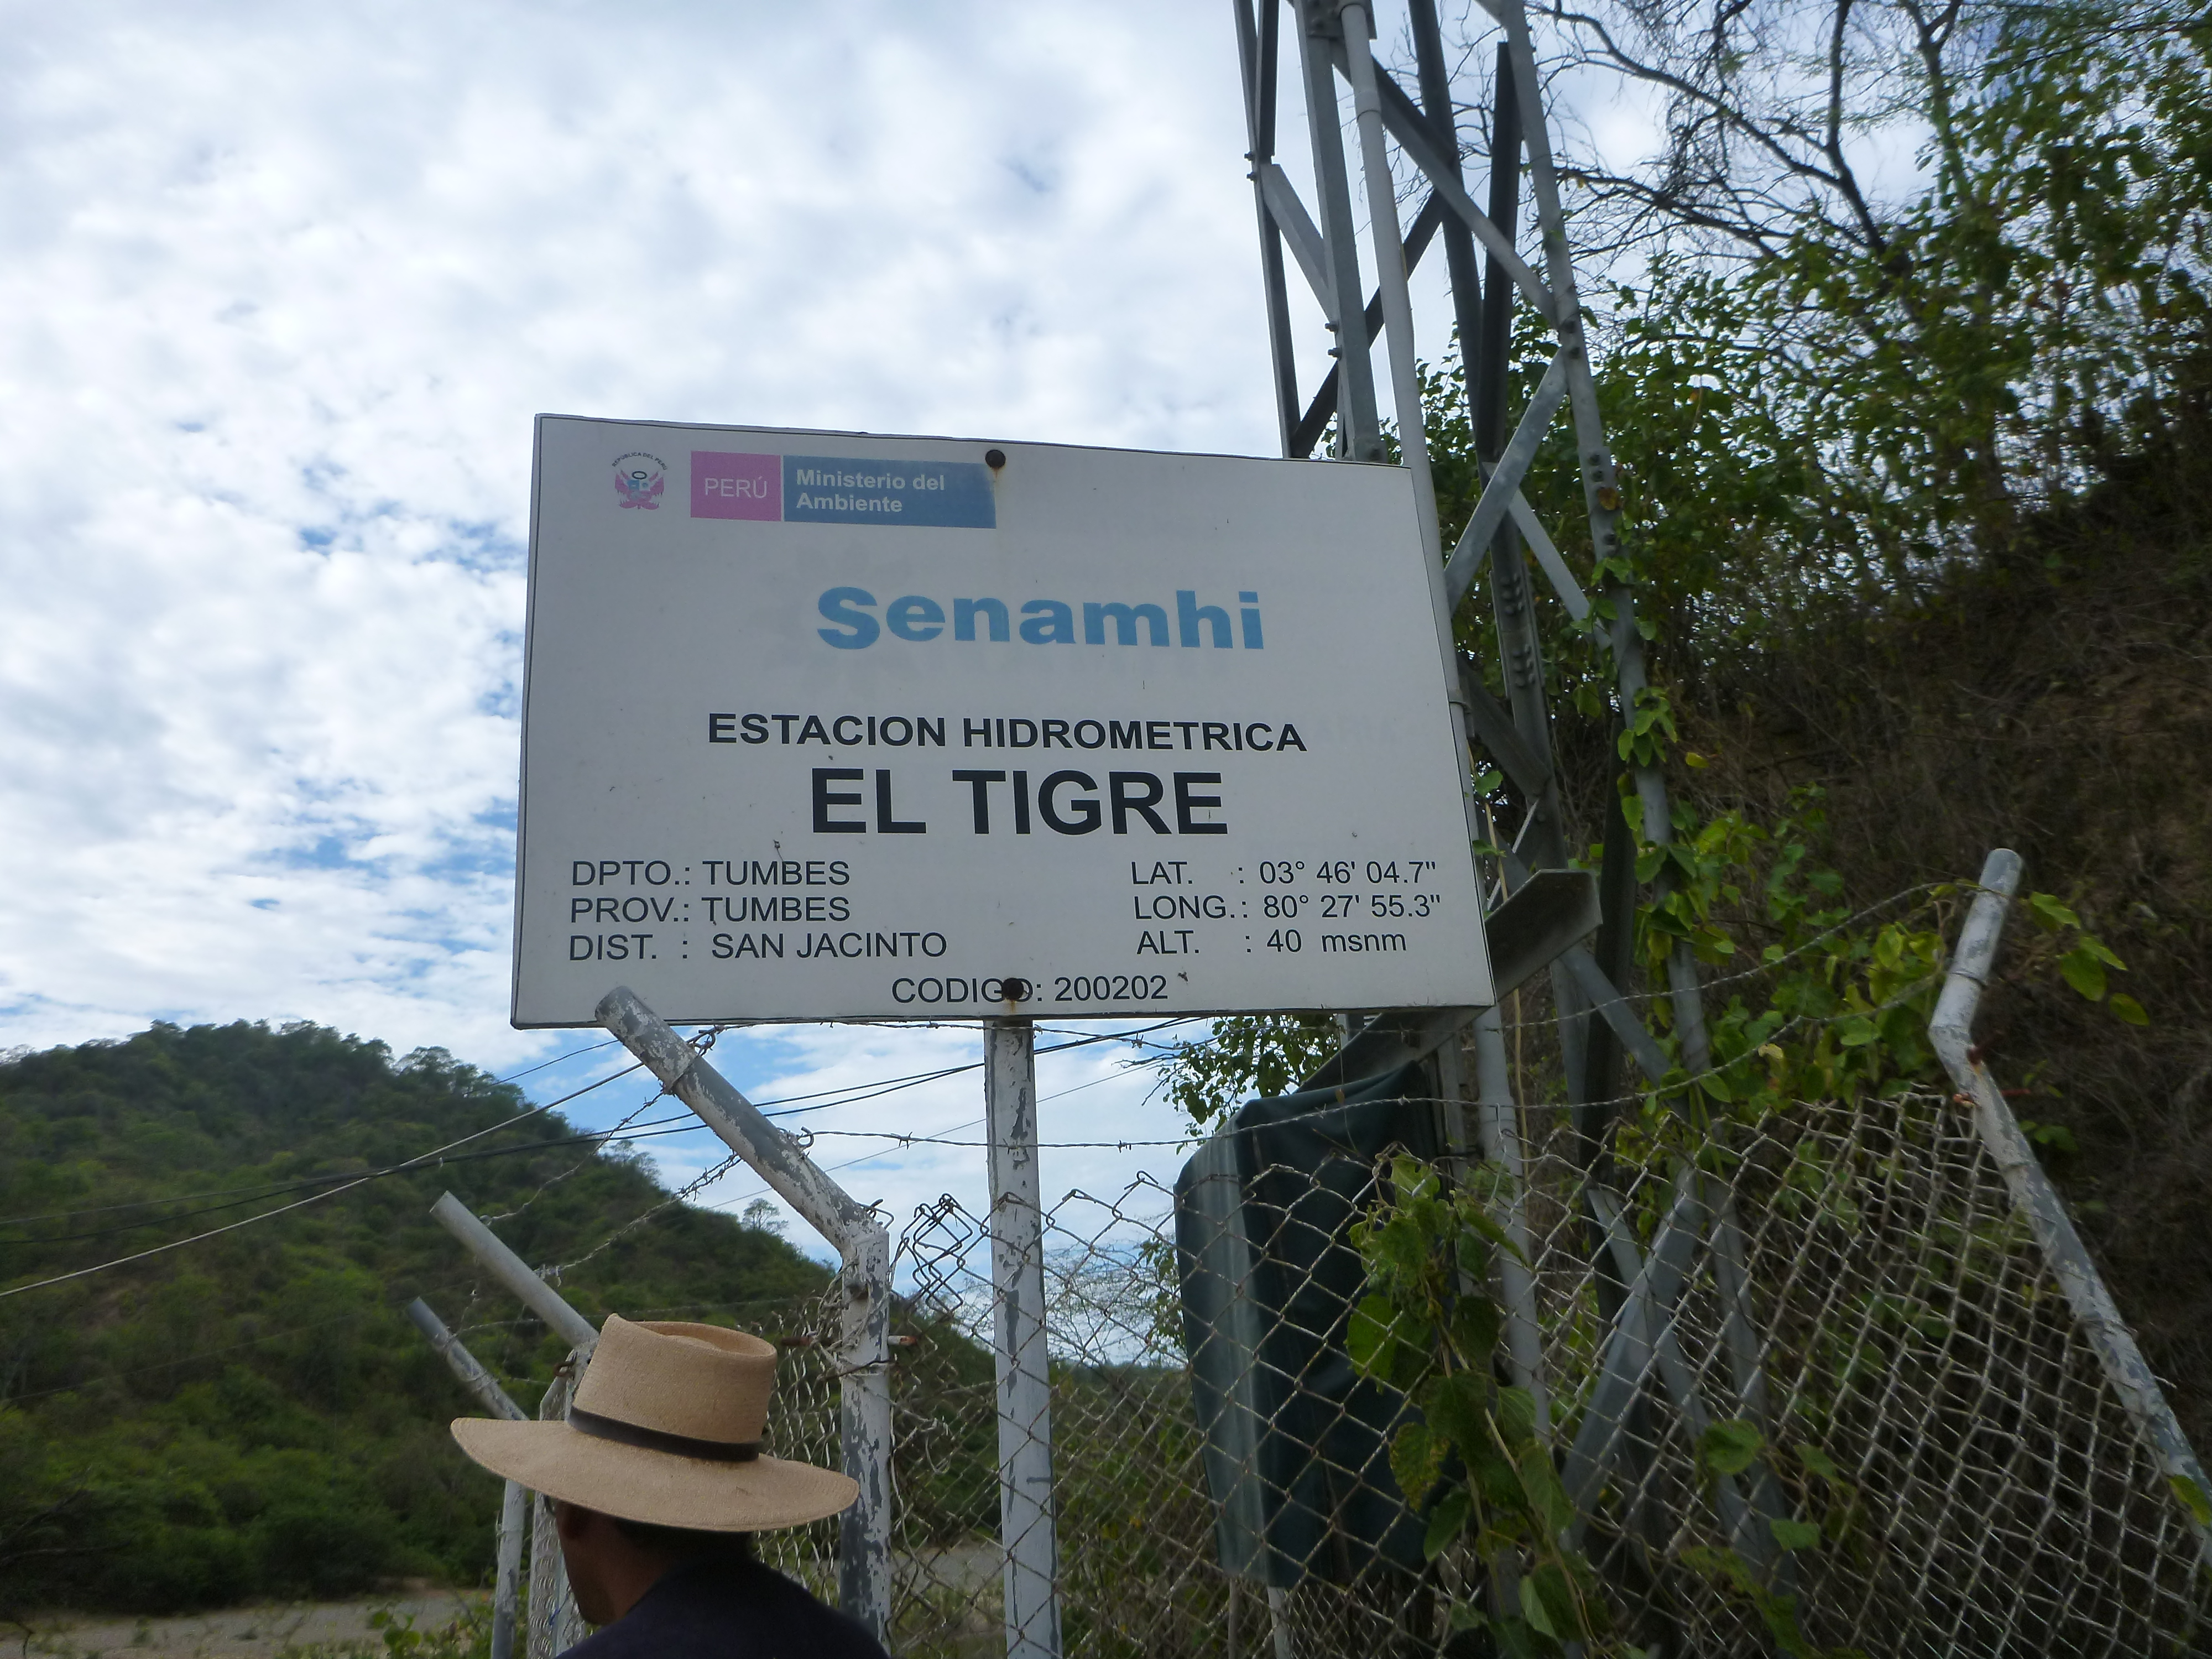
\includegraphics[width=0.5\textwidth]{imagenes/P1040767}
  \caption{Estación hidrológica El Tigre - Rio Tumbes}
  \label{fig:estacion_hidrologica_n01}
\end{figure}

Gracias al proyecto Binacional Puyango-Tumbes tuvimos facilidades para acceder a las tareas de aforo y formar parte de esta en los días 17 y 18 de abril de 2018.\\

\begin{figure}[h]
  \centering
    \includegraphics[width=0.5\textwidth]{imagenes/ubicacionN01}
  \caption{Vista satelital obtenida del Google Maps de la zona de aforo}
  \label{fig:vistaSatelital}
\end{figure}

Para la experiencia se hizo dos tipos de aforo:
\begin{itemize}
\item Aforos líquidos: Se consiguió mediante el uso del equipo ADCP Rio Grande de 1200 khz.
\item Aforos sólidos: Se hizo mediante el aforador vertical triple, integrador de profundidad, Helley Smith y manual.
\end{itemize}

\subsection{Aforos líquidos}
El Riverboat es un dispositivo que permite la instalación en este de los equipos correntometro de efecto Doppler (ADCP) y GPS (Global Positioning System) que se accionan vía frecuencias de radio desde una de las orillas del rio, en la orilla del río también se debe encontrar una persona que desde la laptop hará las lecturas de los datos mediante el uso del software WinRiver II.

\begin{figure}[h]
  \centering
    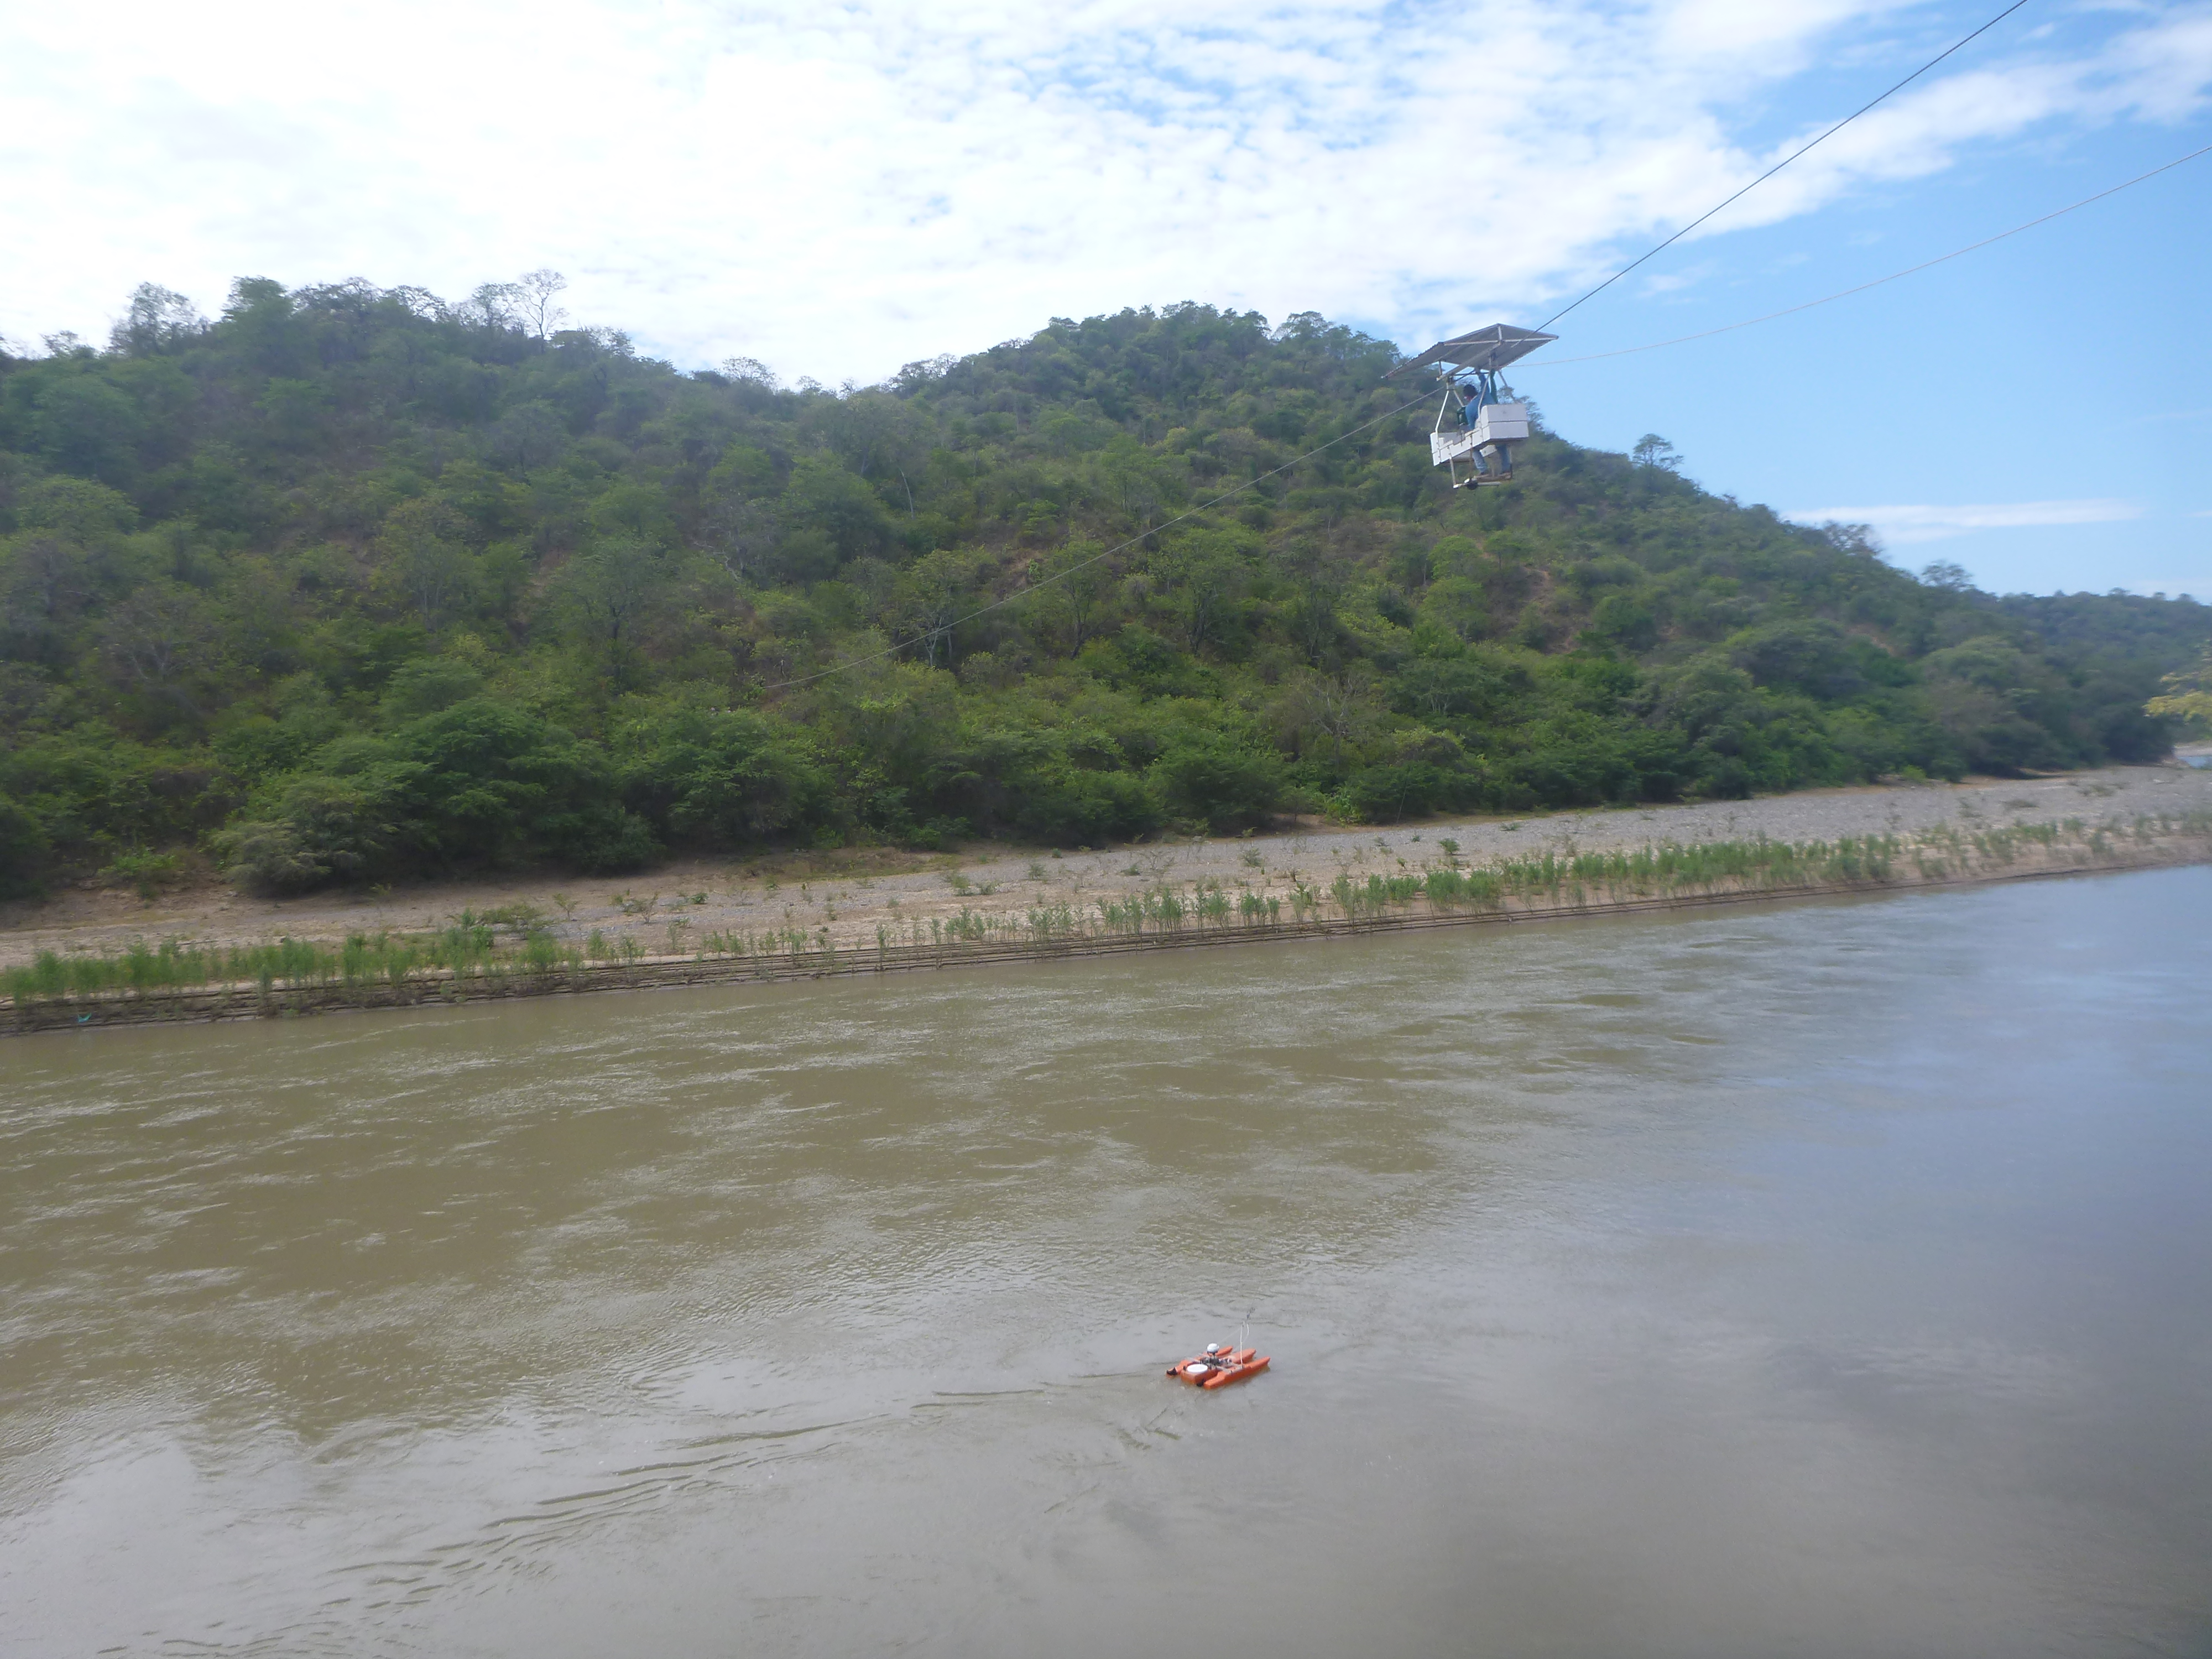
\includegraphics[width=0.5\textwidth]{imagenes/P1040842}
  \caption{Riverboat con ADCP y GPS durante proceso de aforo en rio Tumbes}
  \label{fig:carroAforador}
\end{figure}






Existe un aforador que hace el recorrido en un carro huaro y es esta misma persona la que se encarga de ir desplazando el Riverboat - ADCP WorkHorse Rio Grande 1200 kHz de extremo a extremo del río, a cada recorrido se le denomina transecto, para esta investigación se ejecutaron 4 transectos en cada día de aforo; logrando un total de 2 días de aforo.






\subsection{Aforos sólidos}
Se hicieron aforos estáticos para los puntos fijos en las verticales 35, 50 y 65 metros desde el margen izquierdo del río.

\begin{itemize}
\item Integrador: Permite determinar los sedimentos en suspension en una columa de agua, de mantera homogenia desde la superficie hasta el fondo en la accion de subir y bajar el muestreador. Es un aparato que toma muestras de sedimento en suspensión para una zona puntual, esto se hace para cada punto de aforo; durante el muestro el material en suspensión será almacenada en un recipiente que tiene forma de bebida enlatada ello dentro del pescadito.
\item Muestreador vertical triple: Es un aparato metálico que tiene tres cámaras horizontales, se activa por orden del observador y se cierra inmediatamente dentro del río, luego es retirada y llevada a la orilla para luego verter el contenido en unas botellas de plástico donde serán guardadas y hasta el laboratorio donde se harán los procesos de filtrado.
\item Hally Smith: Permite tomar muestras de sedimentos en el fondo del río, consta de una entrada rectangular de acero y una malla en la parte posterior, al sumergirse este se alinea a la dirección del río y una vez toca fondo empieza a almacenar los sedimentos durante un tiempo determinado en función de la velocidad  para luego ser retirado; las muestras tomadas se poner a secar en posición vertical en el mismo Hally Smith.
\item Manual: Se toma la muestra en la orilla del río con una botella.

\end{itemize}


\begin{figure}[h]
  \centering
    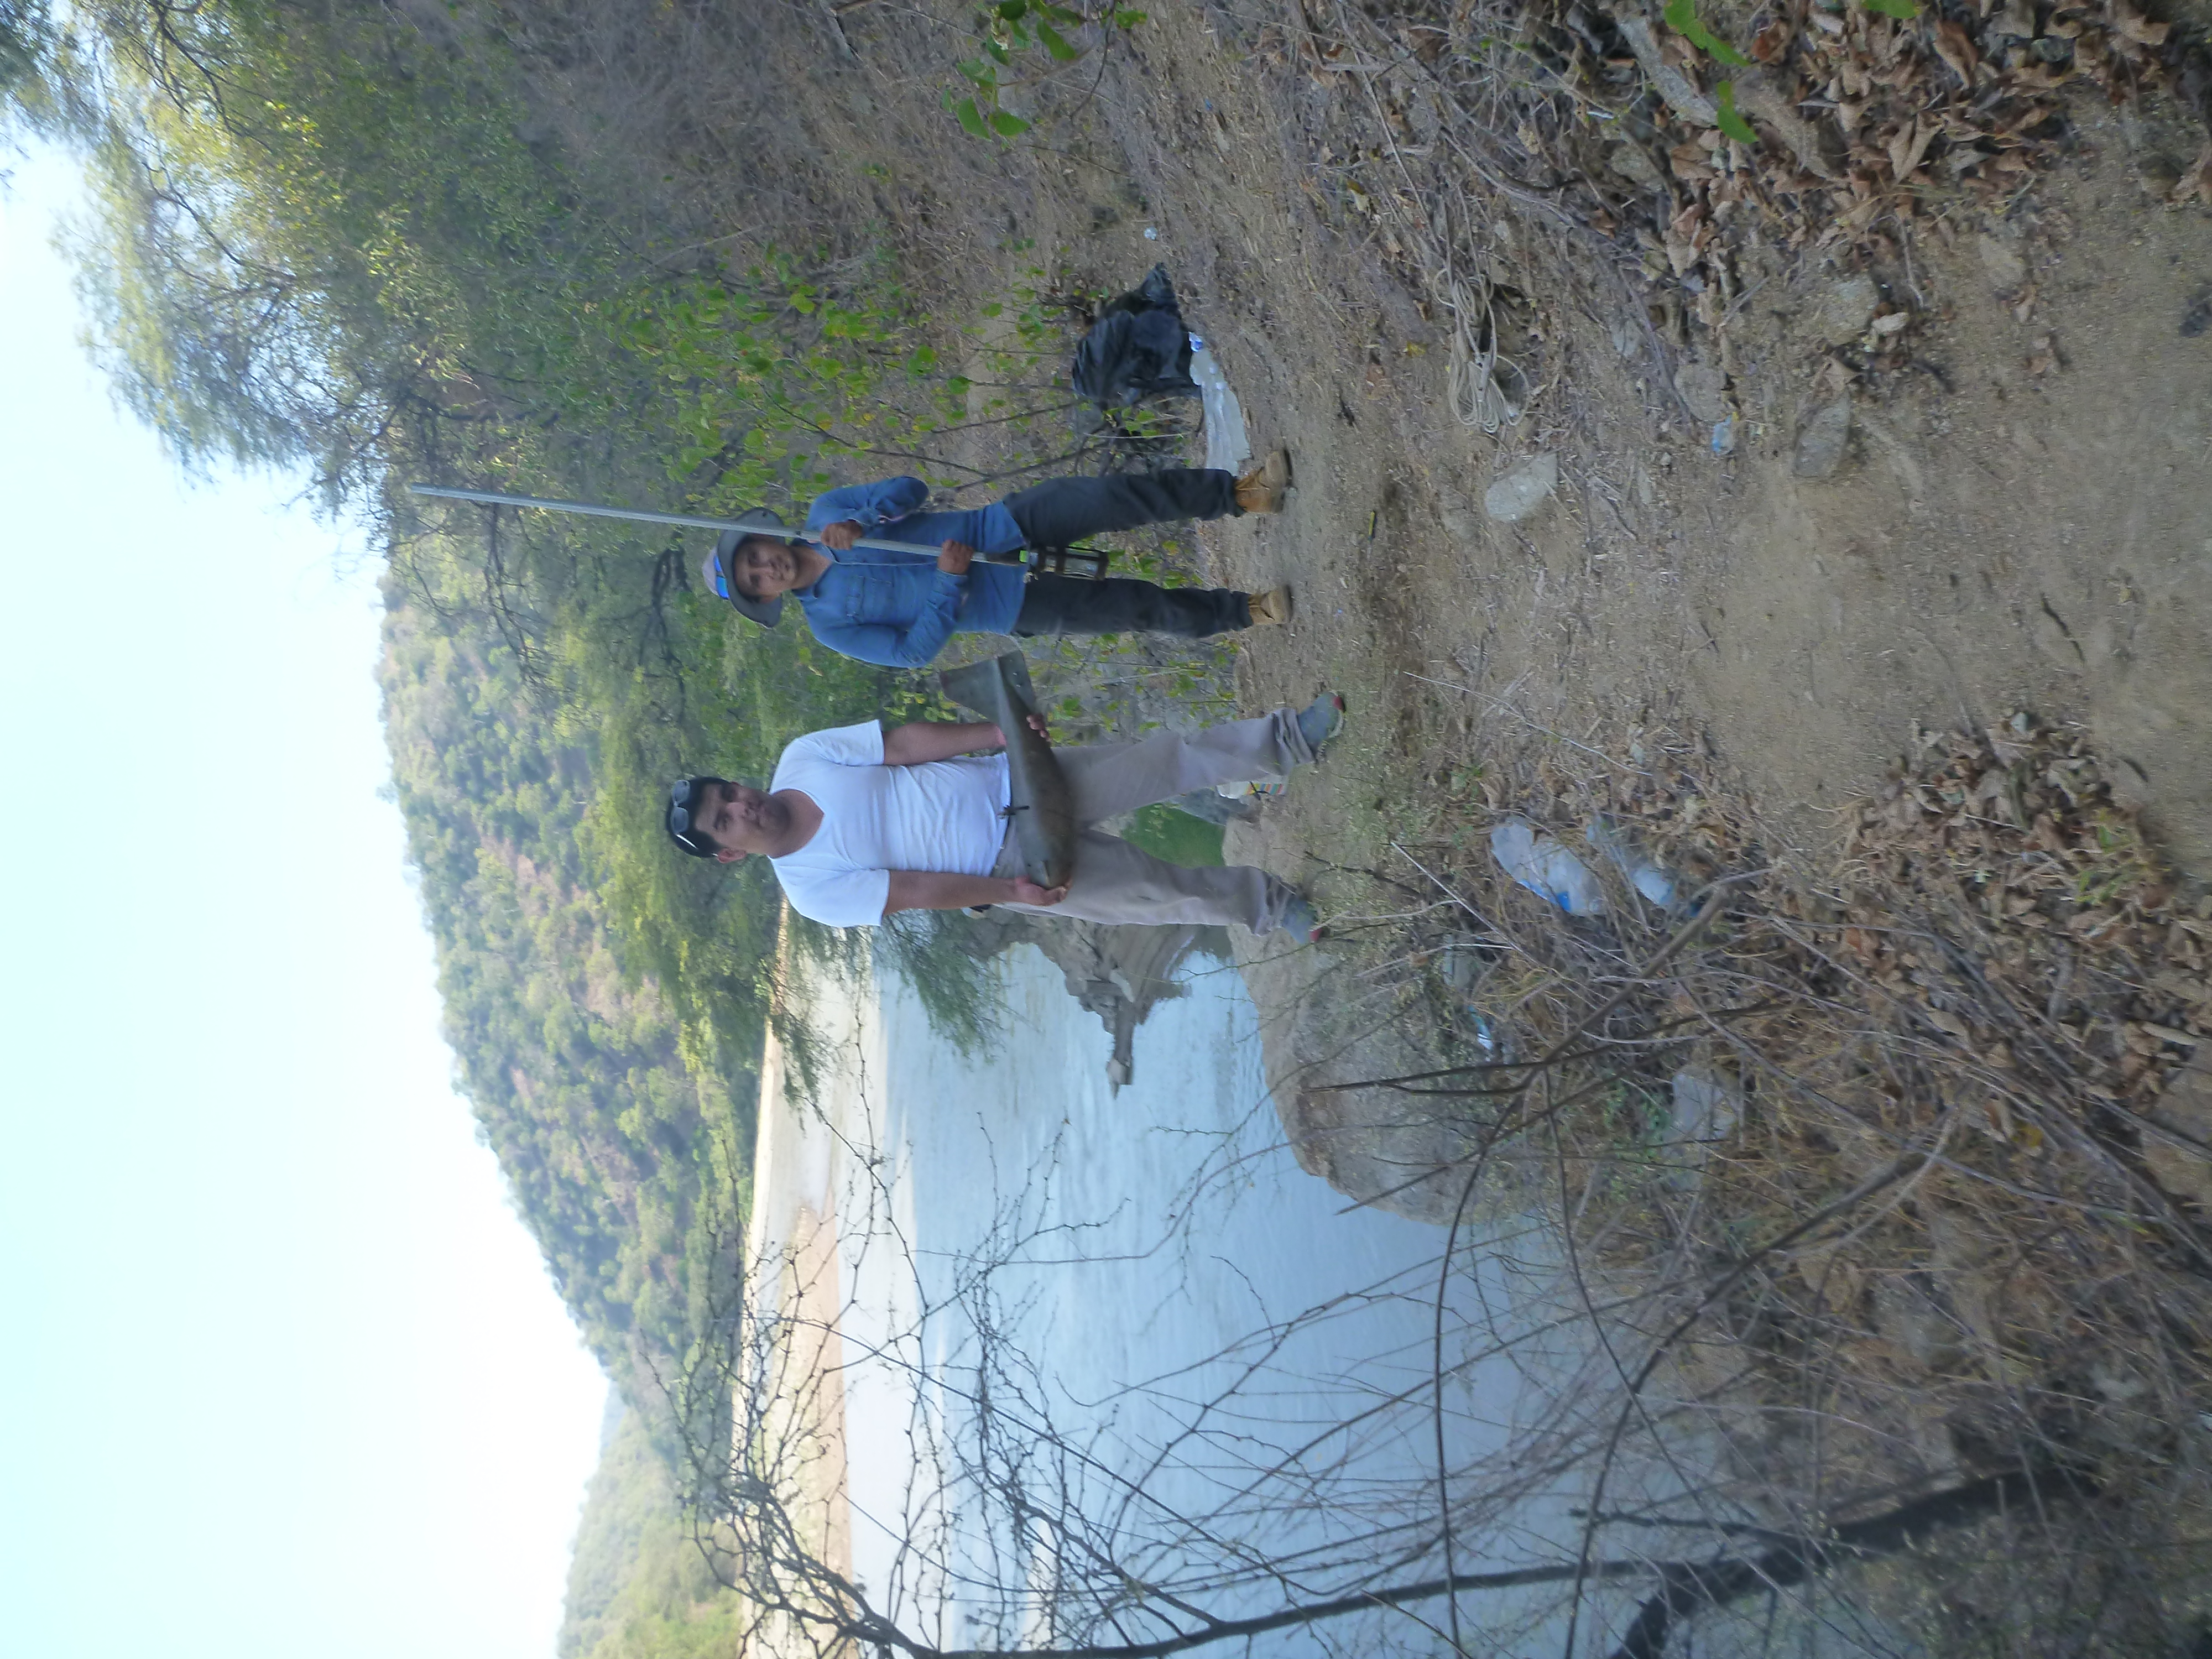
\includegraphics[width=0.5\textwidth]{imagenes/P1050015}
  \caption{Muestreador integrador y el manual de izquierda a derecha de la fotografía tomada en el margen izquierdo del río Tumbes}
  \label{fig:IntegradorPescesitoYManual}
\end{figure}




\subsection{Proceso de muestras de sedimentos}
Esto se logró en el laboratorio de Aguas y Suelos de la facultad de Ingeniería Agricola de la Universidad Agraria La Molina en los meses de abril y mayo de 2018, donde las muestras de solidos aforadas en la estación el Tigre de los días que participamos y de otras fechas se trajo mediante encomienda y ya en laboratorio se comenzó a procesar en los tamises de 100 micras.

\begin{figure}[h]
  \centering
    \includegraphics[width=0.5\textwidth]{imagenes/sedimentos_gruesos}
  \caption{Ejecución de filtrado para sedimetos gruesos}
  \label{fig:FiltroGrueso}
\end{figure}



\subsection{WinRiver II - Formato de salida ASCII}
El software Winriver II permite procesar los datos recolectados por el ADCP (Acoustic Doppler Current Profiler) y almacenarlos en un archivo con extensión .txt ordenandose de la siguiente manera:

% Please add the following required packages to your document preamble:
% \usepackage{multirow}
\begin{table}[h]
\begin{tabular}{|l|l|l|}
\hline
Fila               & Campo & Descripción                                          \\ \hline
A                  & 1     & Comentario 01 sobre el transecto                     \\ \hline
B                  & 1     & Comentario 02 sobre el transecto                     \\ \hline
\multirow{7}{*}{C} & 1     & LONGITUD DE LA CELDA DE PROFUNDIDAD (cm)             \\ \cline{2-3} 
                   & 2     & EN BLANCO DESPUÉS DE TRANSMITIR (cm)                 \\ \cline{2-3} 
                   & 3     & PROFUNDIDAD ADCP DESDE EL NODO DE CONFIGURACIÓN (cm) \\ \cline{2-3} 
                   & 4     & NÚMERO DE CELDAS DE PROFUNDIDAD                      \\ \cline{2-3} 
                   & 5     & NÚMERO DE PINGS POR CONJUNTO                         \\ \cline{2-3} 
                   & 6     & TIEMPO POR CONJUNTO (céntesimas de segundo)          \\ \cline{2-3} 
                   & 7     & MODO DE PERFIL                                       \\ \hline
\end{tabular}
\end{table}

Un segmento viene a ser una fila del archivo ASCII. Las primeras 9 filas traen información que puede ser usada para contar con datos de número de contenedores, fecha y hora, entre otros. En caso se presenten datos erróneos para la velocidad se le asigna un valor de (-32768); para el caudal (2147483647); Latitud y longitud (30000).

% Please add the following required packages to your document preamble:
% \usepackage{multirow}
\begin{table}[h]
\begin{tabular}{|l|l|l|l|}
\hline
Fila                                                                          & Campo & \multicolumn{2}{l|}{Descripción}                                               \\ \hline
\multirow{13}{*}{\begin{tabular}[c]{@{}l@{}}10 - N\\ Segmentos\end{tabular}} & 1     & \multicolumn{2}{l|}{PROFUNDIDAD - (celda de profundidad)}                      \\ \cline{2-4} 
                                                                              & 2     & \multicolumn{2}{l|}{MAGNITUD DE VELOCIDAD}                                     \\ \cline{2-4} 
                                                                              & 3     & \multicolumn{2}{l|}{MAGNITUD DE DIRECCIÓN}                                     \\ \cline{2-4} 
                                                                              & 4     & \multicolumn{2}{l|}{COMPONENTE DE VELOCIDAD ESTE - Este (+) / Oeste (-)}       \\ \cline{2-4} 
                                                                              & 5     & \multicolumn{2}{l|}{COMPONENTE DE VELOCIDAD NORTE - Norte (+) / Sur (-)}       \\ \cline{2-4} 
                                                                              & 6     & \multicolumn{2}{l|}{COMPONENTE DE VELOCIDAD VERTICAL - Arriba (+) / Abajo (-)} \\ \cline{2-4} 
                                                                              & 7     & \multicolumn{2}{l|}{ERROR DE VELOCIDAD}                                        \\ \cline{2-4} 
                                                                              & 8     & \multirow{4}{*}{BACKSCATTER}                      & - Haz 1                    \\ \cline{2-2} \cline{4-4} 
                                                                              & 9     &                                                   & - Haz 2                    \\ \cline{2-2} \cline{4-4} 
                                                                              & 10    &                                                   & - Haz 3                    \\ \cline{2-2} \cline{4-4} 
                                                                              & 11    &                                                   & - Haz 4                    \\ \cline{2-4} 
                                                                              & 12    & \multicolumn{2}{l|}{PORCENTAJE BUENO}                                          \\ \cline{2-4} 
                                                                              & 13    & \multicolumn{2}{l|}{CAUDAL}                                                    \\ \hline
\end{tabular}
\end{table} 



\subsection{Conversión de coordenadas}
Es importante para la geodecía considerar las deformaciones que llegan a presentarse sobre la superficie terrestre y de esta manera se llegó a proponer la creación y utilización de los husos, que vienen a ser divisiones que permiten trabajar en la superfice terrestre, sobre estas han sido dividida en 60 husos, los cuales se comienzan a enumerar desde el meridiano de Greenwich hacia el Este siguiendo la dirección de Sur hacia Norte.

\subsection{Sistema de coordenadas geográficas}
El sistema de coordenadas es el más utilizado ya que su notación es más amigable para el entendimiento humano, consiste en elementos expresados en grados, minutos y segundos.
\begin{itemize}
\item Donde:
	\begin{itemize}
	\item 60 Grados: Representa a la cantidad de husos de la tierra.
	\item 1 Grado: 60 minutos
	\item 1 minuto: 60 segundos
	\end{itemize}
\end{itemize}
Esta distribución se da para la latitud y la longitud.

\subsection{Sistema UTM (Universal Transversal Mercator)}
Las coordenadas UTM son una manera sencilla de representar distancias mediante la combinación de letras y números que se dividen en tres partes del cuerpo, la primera es una combinación de un número y una letra, la segunda representa la latitud y la tercera la longitud, ambas son en metros.

\subsection{Interpolación y ajustes de curva}
Mediante un conjunto de datos discretizados de la forma:

\begin{table}[h]
\begin{tabular}{|l|l|l|l|l|l|l|l|l|l|l|}
\hline
\textbf{x}    & x0    & x1    & x2    & ... &  & ... & x(n-3)    & x(n-2)    & x(n-1)    & x(n)    \\ \hline
\textbf{f(x)} & f(x0) & f(x1) & f(x2) & ... &  & ... & f(x(n-3)) & f(x(n-2)) & f(x(n-1)) & f(x(n)) \\ \hline
\end{tabular}
\end{table}


Se hará uso del método de Newton ya que se cuenta con pocos puntos para el dominio, y en este método a mayor cantidad de puntos para el dominio se tendrá un mayor grado del polinomio; para este método lo primero que se debe hacer es el calculo de la pendiente cuya forma es:

$$ f_{i}(x_{0}, x_{1}, ... , x_{i-1}, x_{i}) = \frac{(f_{i-1}(x_{1}, ... , x_{i-1}, x_{i})) - (f_{i-1}(x_{0}, x_{1}, ... , x_{i-1}) )}{x_{i} - x_{0}} $$

\begin{itemize}
\item Donde:
	\begin{itemize}
	\item $ x_{i} - x_{j} $ es la distancia que hay entre dos elementos.
	\end{itemize}
\end{itemize}

Definiendo el polinomio:
Cuando se cuenta con la pendiente la tarea de definir el polinomio para un grado $n$ se hace mediante el esquema general:

$$ p_{i}(x) = p_{i-1}(x) + f_{i}(x_{0}, x_{1}, ... , x_{i-1}, x_{i})\prod_{j=0}^{i-1}(x-x_{j}) $$


\subsection{Integración mediante el método del trapecio}
El cálculo del área para superficies irregulares podría llegar a representar una tarea algo tediosa sino fueran por las matemáticas, gracias a la integración por el método del trapecio esta se tarea se hace más sencilla, consiste en la división del dominio en muchos pequeñas secciones, de modo que al evaluar las cotas en una función $f(x)$ que describa la curva, bastará con hallár la integral para esta, dando como resultado el área bajo la curva.

La ecucación que ayuda este proceso se expresa de la siguiente manera:

$$ A = \int_{a}^{b} f(x) dx $$
$$A = (b-a)\cdot [\frac{(f(a)+f(b))}{2}]$$


\subsection{Cálculo del caudal para el fluido}
Habiendo obtenido el área de la sección del río mediante la ecuación de continuidad podemos hacer comparaciones de caudales y promediarlos para los transectos hechos durante un aforo.\\

Ya que el campo de velocidades del aforo muestra que estas no son homogeneas la relación de $Q= A * v$ donde Q: Caudal {m3/s}, A: Área {m2}, v: Velocidad {m2/s} , por lo tanto esta ecuación no es solución al problema.

Se hace el cálculo del caudal para velocidades no uniformes mediante la integral:

\[Q = \iint_{a}^{b}v\cdot dS\]

\begin{itemize}
\item Donde:
\begin{itemize}
\item $Q$: Caudal (m3/s)
\item $a, b$: Cotas de los extremos del río en un sistema de referencia.
\item $v$: Velocidad promedio (m/s)
\item $dS$: Vector superfice que se define como $dS = n\cdot dS$ , $n$ es el vecotr unitario normal a la superficie y $dS$ un elemento diferendial de área. (m)
\end{itemize}
\end{itemize}









%%%%%%%%%%%%%%%%%%%%%%%%%%%%%%%%%%%%%%%%%%%%%%%%%%%%%%%%%%%
%%%%%%%%%%%%%%%%%%%%%%%%%%%%%%%%%%%%%%%%%%%%%%%%%%%%%%%%%%%
%%%%%%%%%%%%%%%%%%%%%%%%%%%%%%%%%%%%%%%%%%%%%%%%%%%%%%%%%%%
%%%%%%%%%%%%%%%%%%%%%%%%%%%%%%%%%%%%%%%%%%%%%%%%%%%%%%%%%%%

\section{Resultados esperados}
\begin{itemize}
\item Se espera calcular un valor igual a lo presentado por el WinRiver II para cada muestra transecto.
\item Contar con un software compilado para los sistemas operativos Windows con extensión .exe y para GNU/Linux con extensión .deb .
\item La base de datos debe ser rápida que soporte un total máximo de 50000 registros para ambas tablas.
\item El software debe ser MDI (Multiple Document Interface) desde el menú principal donde se cargaran los submodulos en su interior.
\item Lo resultados gráficos de campo de velocidades , perfil de concentraciones debe tener la opción para almacenarlos en formato .png , .jpg con el fin de que se pueda utilizar para hacer presentaciones de informes técnicos.
\item El método para la interpolación de la sección debe ser la adecuada.
\end{itemize}

\begin{landscape}
\section{Cronograma}
El cronograma se ha desarrollado en función al tiempo que se ha venido trabajando y la estimación para terminar la tesis.
\begin{table}[h]
\begin{tabular}{|l|l|l|l|l|l|l|l|l|l|l|l|l|}
\hline
Tareas\textbackslash{}Meses & Abr & \multicolumn{1}{c|}{May} & Jun                        & Ago & Sep & Oct & Nov & Dic & Ene     & Feb     & Mar    & Abr   \\ \hline
A.Q.L.S.F.M.                  & \multicolumn{2}{c|}{100\%}     &                            &     &     &     &     &     &         &         &        &       \\ \hline
L.B.                        &     &                          & \multicolumn{3}{c|}{100\%}             &     &     &     &         &         &        &       \\ \hline
C.B.D.                      &     &                          & \multicolumn{1}{c|}{100\%} &     &     &     &     &     &         &         &        &       \\ \hline
C.GUI                       &     &                          &                            & \multicolumn{5}{c|}{100\%}  &         &         &        &       \\ \hline
I.F.B.D.B                   &     &                          &                            &     &     &     &     &     & \multicolumn{3}{c|}{100\%} &       \\ \hline
I.R.                        &     &                          &                            &     &     &     &     &     &         &         &        & 100\% \\ \hline
T.S.H.                      &     &                          &                            &     &     &     &     &     &         &         &        & 100\% \\ \hline
E.P.S.O.                    &     &                          &                            &     &     &     &     &     &         &         &        & 100\% \\ \hline
R.M.U.                        &     &                          &                            &     &     &     &     &     &         &         &        & 100\% \\ \hline
\end{tabular}
\end{table}

\begin{itemize}
\item Donde:
	\begin{itemize}
	\item A.Q.L.S.F.M.: Aforo de caudales líquidos y sólidos con el filtrado de muestras para sedimentos.
	\item L.B.: Lectura de la bibliografía propuesta.
	\item C.B.D.: Creación de la base de datos para las tablas de los modulos de laboratorio y campo.
	\item C.GUI: Creación de la interfaz gráfica de usuario.
	\item I.F.B.D.B: Implementación funcional de la base de datos, calculos en el desarrollo del backend.
	\item I.R.: Visualización de resultados gráficos para los campos de velocidad, perfiles de concentración de sedimentos, hidrograma.
	\item T.P.H.: Testing del software hidrosedimentario.
	\item E.P.S.O.: Empaquetado para cada sistema operativo.
	\item R.M.U.: Redacción del manual de usuario.
	\end{itemize}
\end{itemize}


\end{landscape} 


\section{Bibliografía}
\begin{itemize}
	\item Martín. J. (2003). \textit{Ingeniería de ríos}, Mexico: Alfaomega Grupo Editor.
	\item Rocha. A. (1998). \textit{Introducción a la hidráulica fluvial}, Perú: Universidad Nacional de Ingeniería.
	\item Instruments, R. D. (2013). \textit{WorkHorse Rio Grande ADCP User’s Guide}. San Diego, CA.: RI Instruments, 
	\item Instruments, R. D. (2018). \textit{WinRiver II user's guide}, San Diego, CA.: RD Instruments.
	\item Escuidier. M. (2017). \textit{Introduction to Engineering Fluid Mechanics}, Estados Unidos: Oxford University Press.
	\item Gonzáles, R. (s.f.). \textit{Python para todos}. Recuperado de: \textbf{http://mundogeek.net/tutorial-python}
	\item Coutinho, N. (2016). \textit{Introducción a la programación con Python: Algoritmos y lógica de programación para principiantes}, Brasil: Novatec Editora Ltda.
	\item Hill, C. (2016). Learning scientific programming with Python. Estados Unidos: Cambridge University Press.
	\item Harwani, B. (2018). \textit{Qt5 Python GUI Programming Cookbook: Building responsive and powerful cross-platform applications with PyQt}, Estados Unidos: Packt Publishing Ltd.
	\item Owens, M. and Allen, G. (2010). \textit{The Definitive Guide to SQLite}, Estados Unidos: Springer.
	\item Johansson, R. (2015). \textit{Numerical Python}, Estados Unidos: Springer
	\item Carneiro, M. (2007). \textit{Manual de redacción superior}, Perú: Editorial San Marcos E.I.R.L.
\end{itemize}


\end{document}